\documentclass{article}
\usepackage[utf8]{inputenc}
\usepackage[spanish]{babel}
\usepackage{graphicx}
\usepackage{todonotes}
\usepackage{gensymb}
\usepackage[margin=1.25in]{geometry}
\usepackage{titlesec}
\usepackage{titling}
\usepackage{float}
\usepackage{amsmath}
\usepackage{bm}
\usepackage{wrapfig}
\usepackage{enumitem}

\newcommand{\sectionbreak}{\clearpage}
%\newcommand{\subsectionbreak}{\clearpage}
\newcommand{\vc}{\overrightarrow}
\newcommand{\x}{\cdot}

\titleformat{\section}
	{\Huge}
	{}
	{.25em}
	{\filcenter \bfseries}

\titleformat{\subsection}
	{\large}
	{}
	{0em}
	{}[\titlerule]

\titleformat{\subsubsection}
	{}
	{}
	{0em}
	{\bfseries}

\titlespacing{\section}
{0em}
{0em}
{5em}

\titlespacing{\subsubsection} %me permite controlar el espaciado de la seccion que le indico
	{1em}
	{.75em}
	{.5em}
	

\begin{document}
\begin{titlepage}
    \begin{center}
        \vspace*{1cm}
            
        \Huge
        \textbf{Algebra vectorial}
            
        \vspace{0.5cm}
        \LARGE
        Intersección entre planos            
        \vspace{1.5cm}
            
        \textbf{Krapp Ramiro}
            
        \vfill
            
        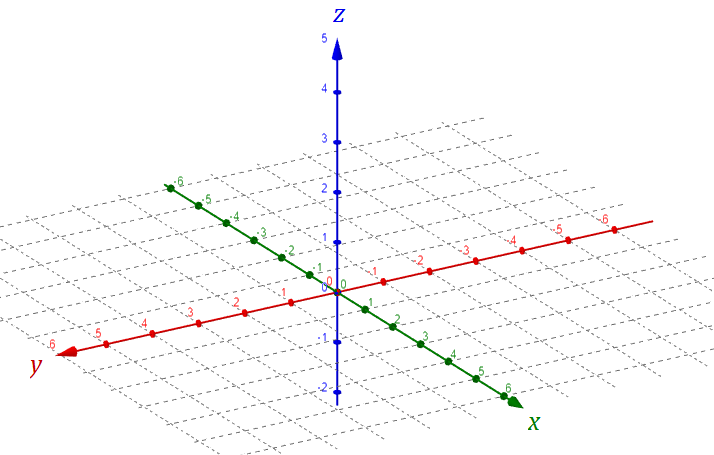
\includegraphics[width=0.8\textwidth]{portada.png}
		  \vspace*{2cm}
            
        \Large
        Instituto Tecnológico San Bonifacio\\
        \today
            
    \end{center}
\end{titlepage}
\section{Actividades}
	\begin{enumerate}
		\item El vector director de la recta resultado de la intersección entre dos planos resultará
			perpendicular a cada uno de los vectores normales que definen los planos.
			Definidos los planos a partir de sus vectores normales, describir:
			\begin{enumerate}[label=\alph*.]
				\item Como obtener el vector director de la recta intersección. (aplicar álgebra vectorial).
				\item Como obtener un punto perteneciente a la recta intersección.
			\end{enumerate}
		\item Con los datos indicados, obtener la expresión cartesiana de:
			\begin{enumerate}[label=\alph*.]
				\item Plano $\pi$ que pasa por Po(-5 , 4, 10) y posee vector normal A (1, -3, 5).
				\item Plano $\alpha$ que pasa por Po(1 , 3, 4) y posee vector normal A (2, 1, 4)
				\item Plano $\beta$ que pasa por Po(2 , 2, 3) y posee vector normal A (-2, 6, -10)
			\end{enumerate}
		\item Obtener la intersección entre:
			\begin{enumerate}[label=\alph*.]
				\item El plano $\pi$ y el plano $\alpha$
				\item El plano $\pi$ y el plano $\beta$ 
			\end{enumerate}

	\end{enumerate}



\section{Ejercicio 1}
	\subsection{a --- Como obtener el vector director de la recta intersección}
		El vector director de una recta intersección es perpendicular a los dos planos, es un vector que resulta perpendicular
		al plano en el cual estan localizados los planos.

		Para averiguarlo, hay que hacer un producto vectorial.
	\subsection{b --- Como obtener un punto perteneciente a la recta intersección.}
		Para obtener un punto perteneciente a la recta, hay que multiplicar cualquier valor, llamemoslo $\alpha$, 
		por el vector director $\vc{A}$ de la recta, y se le suma el punto de origen $P_0$

		Esto está en el apunte como $Q = P_0 + \alpha \x \vc{A}$

\section {Ejercicio 2}
	\subsection{a --- Plano $\pi$ que pasa por $P_0 (-5,4,10)$ y posee vector normal $\vec{A}(1,-3,5)$}
			$
			\vc{A} \cdot \vc{P_0 -P} = 0 \\
			1\x (-5-x) -3\x (4-y) +5\x (10-z) = 0 \\
			-5-x ~ -12+3y ~ +50-5z = 0\\
			-33 = -1x+3y-5z \quad\longrightarrow\quad \boldsymbol{33 = x-3y+5z : \pi} \\
			$
	\subsection{b --- Plano $\alpha$ que pasa por $P_0 (1,3,4)$ y posee vector normal $\vec{A} (2,1,4)$}
			$
			\vc{A} \cdot \vc{P_0 -P} = 0 \\
			2\x (1-x) + 1\x (3-y) + 4\x (4-z) = 0 \\
			2-2x + 3-y + 16-4z = 0 \\
			-2x -1y -4z = -21 \quad\longrightarrow\quad \boldsymbol{2x+y+4z = 21 : \alpha} \\
			$
	\subsection{c --- Plano $\beta$ que pasa por $P_0 (2,2,3)$ y posee vector normal $\vec{A} (-2,6,-10)$}
			$
			\vc{A} \cdot \vc{P_0 -P} = 0 \\
			-2\x (2-x)+6\x (2-y) -10\x (3-z) \\
			-4+2x ~+~ 12-6y ~+~ 30-10z = 0 \\
			\boldsymbol{2x -6y +10z = 22 :\beta} \\
			$

\section{Ejercicio 3}
	\subsection{a --- Obtener la intersección entre el plano $\pi$ y el plano $\alpha$}
		\begin{center} \textbf{Calculo del vector director de la recta} \end{center}
			Planos: \\
			$
			\pi	: 1x - 3y + 5z = 33 \\
			\alpha: 2x + 1y + 4z = 21 \\\\
			\begin{vmatrix}
			i & j & k \\
			1x & -3y & 5z \\
			2x & 1y & 4z
			\end{vmatrix}
			\longrightarrow (-3\x4 - 5\x1)i ~+~ (5\x2 - 1\x4)j ~+~ (1\x1 - -3\x2)k  \\
			$
			\[\boldsymbol{-17i + 6j + 7k} \]
			\vspace*{0.15cm}

		\begin{center} {\textbf{Calculo de punto de origen}} \end{center}
			$
			\text{Considerando } x = 0 \\
			-3y +5z = 33 \\
			1y +4z = 21 \\ \\
			%
			\Delta_s\begin{vmatrix}
				-3 & 5~ \\
				1 & 4~ \\
			\end{vmatrix} \longrightarrow -12 -5 = -17 \\
			\Delta_1\begin{vmatrix}
				33 & ~5~\\
				21 & ~4~\\
			\end{vmatrix} \longrightarrow 132 - 105 = 27 \\
			\Delta_2\begin{vmatrix}
				-3 & 33 \\
				1 & 21 \\
			\end{vmatrix} \longrightarrow -63 - 33 = -96 \\\\\\
			%
			y = \dfrac{\Delta_1}{\Delta_s} = \dfrac{27} {-17} = 1,588 \\\\
			z = \dfrac{\Delta_2}{\Delta_s} = \dfrac{-96}{-17} = 5,647 \\\\
			\text{Origen : } 0x,~ 1,58y,~ 5,64z \\
			$


			\begin{figure}[H]
				\centering
				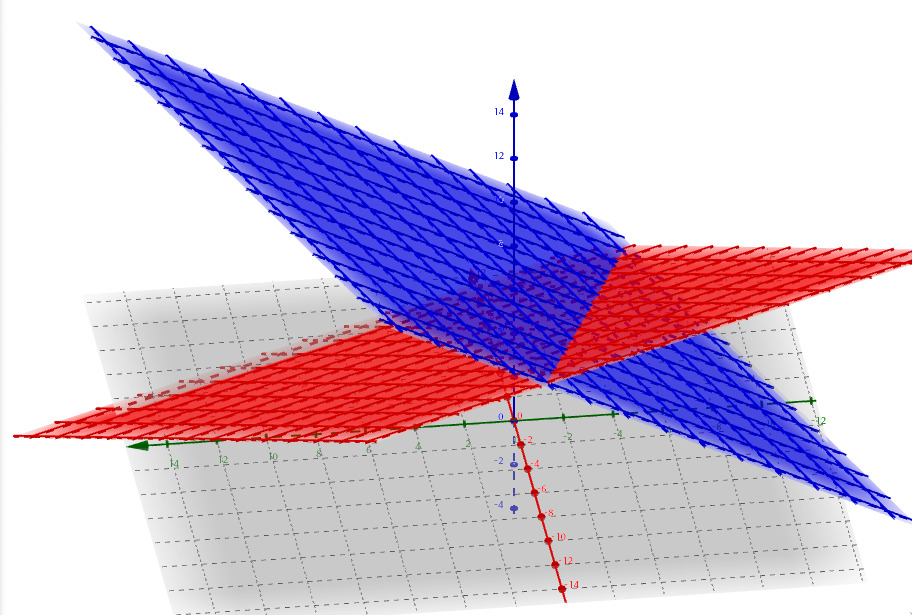
\includegraphics[width=0.4\textwidth]{grafico1.jpg}
			\end{figure}
			\newpage

	\subsection{b --- Obtener la intersección entre el plano $\alpha$ y el plano $\beta$}
		\begin{center} \textbf{Calculo del vector director de la recta} \end{center}
			Planos: \\
			$
			\pi	: 1x - 3y + 5z = 33 \\
			\beta	: 2x -6y +10z = 22 \\\\
			\begin{vmatrix}
				i & j & k\\
				1x &-3y &5z\\
				2x &-6y &10z\\
			\end{vmatrix}
			\longrightarrow (-3\x10 - 5\x-6)i + (5\x2 - 1\x10)j + (1\x-6 - -3\x2)k
			$
			\[\boldsymbol{0i + 0j + 0k} \]

			Como el resultado del producto vectorial da 0 en i, j \& k, se deduce que los planos son paralelos, o sea que \emph{nunca se cruzan}. 
			\begin{figure}[H]
				\centering
				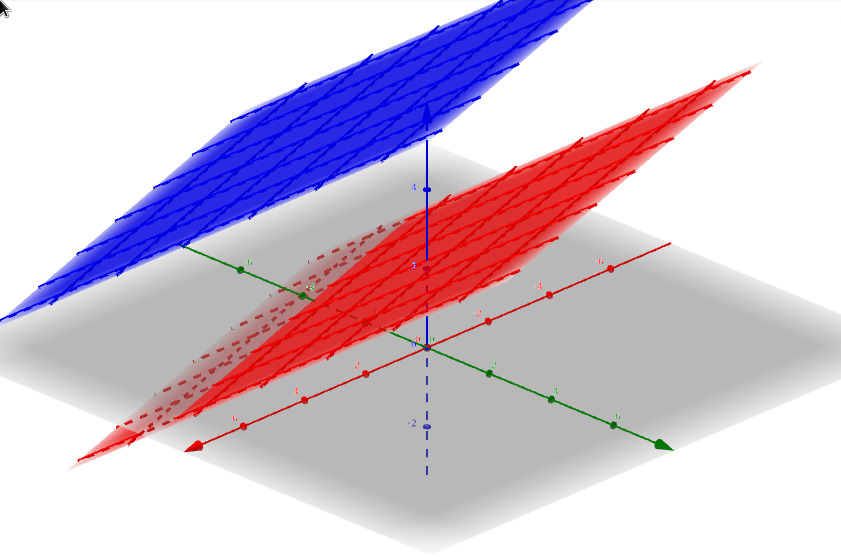
\includegraphics[width=0.7\textwidth]{grafico2.jpg}
			\end{figure}
\end{document}
